% !TeX spellcheck = en_US
% !TEX root = ../thesis.tex

\chapter{Introduction} \label{ch:introduction}

\section{Overview}

\subsection{Early artificial intelligence references}
Humans are curious by nature. We have the desire to understand everything around us, from the smallest particle to the vastness of the universe. Our quest for knowledge is what has allowed us to progress as a species and keep evolving. In this journey, we have always looked up at the stars, dreaming of discovering other intelligent beings like us. In this search, we have also looked inward, trying to understand our thoughts, emotions, and the source of our intelligence and consciousness. 

Since ancient times, the human being has dreamed of artificial intelligence (AI). One of the first existing records dates back to \textit{Aristotle} (384–322 BCE) in his book \textit{The Politics}, where the author imagined machines that would think by themselves and act autonomously, with the purpose of allowing humans enjoy leisure \autocite{nils2009}. In 10-70 CE, the mathematician and engineer \textit{Hero of Alexandria} designed several ancient automata \autocite{greenwood1851}, among which stands out an automated theater that would play short performances in front of the audience.

In the 9th century, the three Persian brothers known as \textit{Banū Mūsā} wrote the \textit{book of ingenious devices} \autocite{musa1978}. In their book, they illustrated hundreds of automata along with other mechanical devices (timing and delay devices, automated valves, etc.) and described how those would be used. 

The philosopher, scientist and bishop \textit{Albert Magnus}, in the middle ages (13th century), manufactured several automata. One of the most notorious ones was an artificial talking head able to imitate human voice and breath \autocite{worthies1828}.

Later on, in the renaissance (15th century), the polymath \textit{Leonardo da Vinci} sketched various automata \autocite{nils2009}. His mechanical knight is one of the first anthropomorphic automata we have record of. This automaton was designed to perform basic human-like motions through a system of pulleys and cables. More recently, these sketches have been studied and the mechanical knight has been built faithfully following the original design \autocite{elling2006}, finding that the automaton was fully functional. 

During the 18th century, automata reached a new level of sophistication, the modern history becoming the golden era of automata. One of the most prolific creators was the watchmaker \textit{Pierre Jaquet-Droz} (18th century), who built a number of automata, including a three-year-old child that could write any letter of the alphabet \autocite{carrera1979}.

Years later, other illustrious automata builders of the era were \textit{Wolfgang von Kempelen} (1734-1804), who built \textit{the Turk}, an automaton that could beat any human at chess\footnote{Although after his death, it was discovered that it was actually nothing more than a machine operated by a person from inside a wooden cabinet.} \autocite{jay2000}, 
and \textit{Jacques de Vaucanson} (1709-1782), who built a number of automata, including a duck that could eat and drink \autocite{nils2009, trymbaka2022}. Despite the complexity and ingenuity gained over the years, these automata were all purely mechanical and human operated, without any form of artificial intelligence. 

Fiction stories have often been used as a way to explore the idea of artificial intelligence, and the earliest references in literature date back to the middle ages. In \textit{The City of Brass}, one of the tales included into the \textit{One Thousand and One Nights} (around the 10th century), the main character, a thief, comes across a city ruled by a wizard who created a brass humanoid automaton that could talk and move like a human. In the 19th century, \textit{E.T.A. Hoffmann} (1776-1822) wrote a story entitled \textit{The Sandman} \autocite{hoffmann1816}, where the protagonist falls in love with an automaton created by a professor, without realizing that she was actually a machine. He suffered a mental breakdown after finding out. This automaton, known as \textit{Olympia}, was able to move, talk and sing. In one of the most famous science fiction novels of all times, \textit{Frankenstein}, written by \textit{Mary Shelley} in 1818 \autocite{shelley1994}, the scientist \textit{Victor Frankenstein} creates a human-like creature out of body parts of different people. Although, strictly speaking, \textit{Frankenstein}'s creature is not a machine, it is often seen as one of the first examples of intelligent creations in literature.

A century later, the Czech writer, playwright and critic \textit{Karel Čapek} (1920), wrote a play named \textit{R.U.R.} (\textit{Rossum’s Universal Robots}), which is considered to be the first recorded use of the term \textit{robot}\footnote{The word \textit{robot} is derived from the Czech word \textit{robota}, which means forced labour or slaves.}  \autocite{nils2009}. In that play, robots were manufactured as slaves to do the manual labour that humans disliked. This is often seen as the beginning of the modern science fiction genre.

In 1941, the science fiction writer \textit{Isaac Asimov} published a short story called \textit{Runaround} \autocite{nils2009}, in which he introduced the three laws of robotics (depicted below), which are still considered the basis for the ethical design of robots.

\begin{enumerate}
	\item \textit{A robot may not injure a human being or, through inaction, allow a human being to come to harm}.
	\item \textit{A robot must obey the orders given to it by human beings, except where such orders would conflict with the First Law}.
	\item \textit{A robot must protect its own existence as long as such protection does not conflict with the First or Second Law}.
\end{enumerate}

The above examples are only a few of the many references to artificial intelligence that have been made over the years \autocite{nils2009}. Even though none of these automata were truly intelligent, they represent the beginning of the long and arduous process of building machine intelligence.  

The yearning for artificial intelligence has come and gone in waves over the years, but it has never lost its appeal to human imagination. Each time a new wave of artificial intelligence hits, it brings with it renewed enthusiasm for the possibility that machines can think and act by themselves. 

Recently, artificial intelligence has begun to show significant promise for actually becoming a reality. The history of artificial intelligence is a long one, and its future is still to be written.

\subsection{Modern artificial intelligence}
The dream of AI started to become a reality in the 20th century, with the development of the first computers. In the 1950s, the idea of artificial intelligence was rediscovered by \textit{Alan Mathison Turing} (1912 - 1954), today known as the father of computer science. He secretly defeated the German intelligence's cryptography system (\textit{Enigma} machines; \citealp{Hodges:2000}) and provided a proof showing that it was not possible to find a general solution for the \textit{Hilbert's Entscheidungsproblem} (an important symbolic logic challenge; \citealp{turing1936}). Later, he published the famous article entitled \textit{Computing Machinery and Intelligence} \autocite{turing1950} in which he described a game as a test for machine intelligence. The currently known as \textit{Turing test} consists of an interrogation between a human and an entity (that can either be another human or a machine). The human interrogator's objective is to try to determine, by asking a series of questions, whether the entity it is talking to is a human or a machine. If the interrogator cannot tell the difference (70\% of the times after multiple 5 minutes conversations), then the machine is said to have passed the test, and hence it can be considered intelligent.


The ``artificial intelligence'' term was not coined until 1956 when \textit{John McCarthy} (1927 - 2011) \textit{Nathaniel Rochester} (1919 - 2001) and \textit{Claude Shannon} (1916 – 2001) gave a conference at \textit{Dartmouth College} proposing a 2 month workshop, called the \textit{Dartmouth Summer Research Project on Artificial Intelligence}. This workshop was organized to fund the artificial intelligence as an academic discipline (see the picture in figure \ref{fig:dartmouth_photo}) and the project was fundraised by the \textit{United States Office of Naval Research}. This historical event brought together some of the most prominent computer scientists of the time, including \textit{Marvin Minsky} (1927–2016), \textit{Arthur L. Samuel} (1916–1990), \textit{Ray Solomonoff} (1926-2009) and  \textit{John Nash} (1928-2015), between others\footnote{\textit{John McCarthy}, \textit{Claude Shannon}, \textit{Trenchard More}, \textit{Nathaniel Rochester}, \textit{Oliver Selfridge}, \textit{Julian Bigelow}, \textit{W. Ross Ashby}, \textit{W.S. McCulloch}, \textit{Abraham Robinson}, \textit{Tom Etter},  \textit{David Sayre}, \textit{Kenneth R. Shoulders}, \textit{Alex Bernstein}, \textit{Herbert Simon} and \textit{Allen Newell}.}.

\begin{figure}[h!]
	\centering
	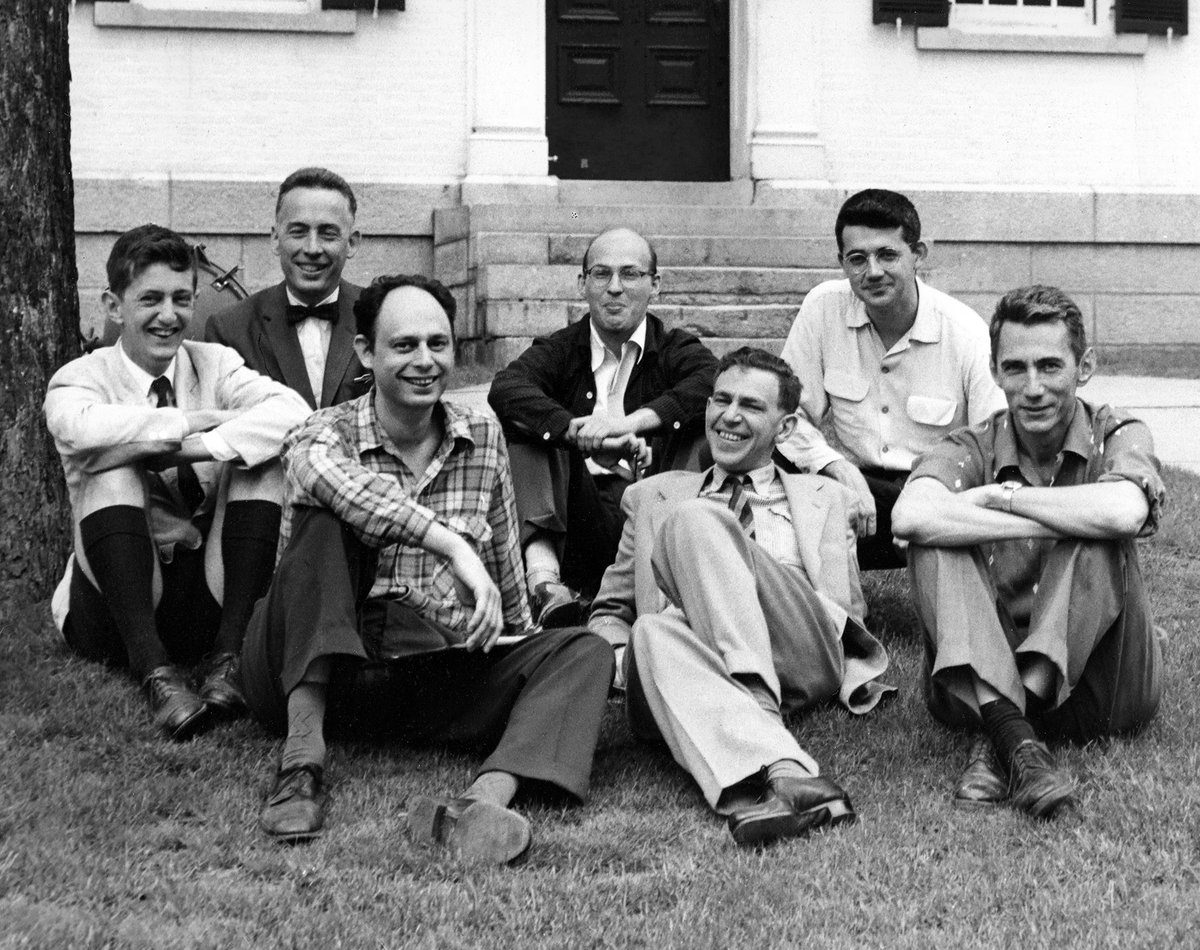
\includegraphics[width=.6\textwidth]{introduction/images/dartmouth}
	\caption[\textit{Dartmouth Summer Research Project on Artificial Intelligence}]{From left to right: \textit{Oliver G. Selfridge}, \textit{Nathaniel Rochester}, \textit{Ray Solomonoff}, \textit{Marvin Minsky}, \textit{Trenchard More}, \textit{John McCarthy} and \textit{Claude Shannon} at the \textit{Dartmouth Summer Research Project on Artificial Intelligence} (Photo: \textit{Margaret Minsky}).}
	\label{fig:dartmouth_photo}
\end{figure}

The recent development of artificial intelligence has not been a linear process and, during its evolution, there have been ups and downs along the way, with several so-called \textit{AI winters}. The \textit{first AI winter} took place between the late 1970s and early 1980s, when research on artificial intelligence came to a standstill. Later, \textit{Sir James Lighthill}, a well-known British scientist, published a report, today known as \textit{the Lighthill report}, concluding that artificial intelligence was a waste of time and money \autocite{lighthillReport}. This publication, together with the oversized expectations for artificial intelligence at the time \autocite{russellNorvig}, led to a decrease of investment for AI research. As a result, the field of artificial intelligence went into decline, stalling for several years.

After the first \textit{AI winter}, the field experienced a revival when several companies started investing in the development of \textit{expert systems}\footnote{A rebranded form of artificial intelligence.}. Software and hardware companies such as \textit{Teknowledge} and \textit{LISP Machines Inc.} grew rapidly during this time in order to meet the rising demand for artificial intelligence technology, which motivated the AI research community to continue with their work. One of the most remarkable inventions of the 80s was the successful application of the \textit{backpropagation} algorithm to neural networks by \textit{David Rumelhart} and \textit{Geoffrey Hinton} \autocite{hinton1986}, which revived the study of artificial neural networks. All this sudden success, together to the collapse of \textit{LISP Machines Inc.} in 1987, led to the \textit{second AI winter}.

The 1990s started with a renewed interest in artificial intelligence and, motivated by the increasing computational power, machine learning algorithms started to be applied to a wider range of tasks \autocite{Tesauro:1995}. Many interesting applications were developed during that decade across several industries like medical diagnosis \autocite{declaris1991, Klein1991, punch1992, Cinar1999}, psychology \autocite{Dorrer1995, denby1999, Ogawa1999, Perlovsky1999}, finance and logistics \autocite{Lipshutz1991, Benaroch1991, Johnson1991, Falas1994} and many others \autocite{Smithers1993, Yoo1994, Mashaly1994, Koyma1998}. Finally, the most sounded event of the 1990s was the victory of the IBM super-computer \textit{Deep Blue} \autocite{Campbell2002} over \textit{Garry Kasparov}, the world chess champion, which took place in \textit{New York City} in 1997. In 1998, \textit{Yann Lecun} and his collaborators published their work on convolutional neural networks \autocite{lecun1999}, a fundamental advance in machine learning which has been widely used in computer vision and other fields. 

The beginning of the 21st century is one of the most fruitful periods for artificial intelligence, with several major achievements in different areas. Further research in neural networks \autocite{hinton2006, hinton2012} gave birth to novel techniques that allowed training deeper models, leading to a rebranding of neural networks as deep learning. In 2011, \textit{IBM's} artificial intelligence program \textit{Watson} won the quiz game \textit{Jeopardy!} against two of the best human players of all time. 

In 2012, \textit{AlexNet} \autocite{krizhevsky2012}, a deep learning model developed by \textit{Geoffrey Hinton} and his collaborators, achieved state-of-the-art performance on the \textit{ImageNet} classification task \autocite{ILSVRC15}, kickstarting the current deep learning revolution. 

In 2016, \textit{Google's} artificial intelligence program \textit{AlphaGo} \autocite{silver2016} defeated the world champion \textit{Lee Sedol} in \textit{the game of Go}, a feat that was considered impossible a few years earlier, by using \textit{reinforcement learning} algorithms. \textit{Alpha Go Zero}, the \textit{Alpha Go's} big brother, proved in 2017 to be more powerful than its predecessor while not needing human interaction to learn \autocite{Silver2017a, Silver2017b}. In 2016, \textit{DeepMind} researchers published \textit{WaveNet} \autocite{vanderoord2016}, a deep auto-regressive model that was able to produce natural raw audio waveforms faithfully generating human speech (a modern version of \textit{WaveNet} has been used in the experiments described in chapter \ref{ch:tts}). One year later, the authors of \citet{vaswani2017} published the transformer, a new architecture designed for sequence transduction tasks that allowed parallel training, as opposed to its sequence-to-sequence predecessors \autocite{sutskever2014}. The transformer architecture has been used in the experiments described in chapter \ref{ch:salesforecast}. In 2020, \textit{OpenAI} researchers published \textit{GPT-3} \autocite{brown2020}, a massive neural network with 175 billion parameters which was able to achieve strong performance on many NLP tasks\footnote{A live example of the power of this model can be found in some of the lines of this chapter, which have been revisited and rephrased with its help.}. Later, in 2021, \textit{AlphaFold} was published by \textit{DeepMind} researchers \autocite{Jumper2021} as a method for inferring the 3D structure of a biological protein based on its genetic sequence, representing one of the major contributions of artificial intelligence to scientific discovery. Finally, in 2022, \textit{OpenAI} researchers published \textit{Dall-e 2}, a text to image generation model able to generate high quality images from textual descriptions \autocite{aditya2022}.

In addition to the mentioned achievements, many algorithms have been published in the generative modeling field. Generative adversarial networks \autocite{Goodfellow2014}, variational auto-encoders \autocite{kingma2019}, normalizing flows \autocite{kingma2016, kobyzev} and diffusion models \autocite{Prafulla2021} are some of the most remarkable examples. Some of these techniques will be discussed in detail in section \ref{sec:generative}.

Many more advances have been made in AI in the past few years, which has led to an increased interest in the technology from both the private and public sectors. However, the application of artificial intelligence to the most complex and important problems still faces many challenges. Here is where deep learning comes into play, as it has shown the ability to achieve state-of-the-art results on a wide range of tasks. Therefore, the development of democratized and low-resource deep learning applications is essential for the future of artificial intelligence. 

Many of the last advances in the deep learning research community report prohibitive amounts of computation needed to train deep learning models \autocite{silver2016, kechyn2018, brown2020, floridi2020}. The authors of \autocite{strubell2019} estimated the amount of $CO_2$ emissions from training a large transformer network (\textit{BERT} size) to be equivalent to the emissions of 5 average cars during all their lifetime, or those of a human during 60 years. 

Research in low-resource deep learning \autocite{howard2017, Han2017, Gao2018, sanchez2020, so2021} has shown the possibility of training deep learning models with a low amount of computation, and its necessity for the future of artificial intelligence, as well as for our planet health.


\section{Contributions}
This dissertation encompasses five contributions to the state of the art of the field of deep learning. Two of them contribute around training methods, and the remaining three are examples of novel applications of deep learning algorithms to industry problems. All the contributions are related to the efficient use of computational resources. Each of these studies is written as a different chapter.

The first contribution (chapter \ref{ch:modulus}) proposes a new activation function for deep learning models: the \textit{modulus} function. The experiments conducted show that, in line with the current research trends, non-monotonic activation functions generally produce better results than monotonic ones. Additionally, the \textit{modulus} activation function is very efficient to compute, as it consists of a single-bit operation, and its derivative (being either 1 or -1) has constant 1-norm. These properties are specially useful for embedded applications. Moreover, the results show that the proposed activation function achieves superior results in computer vision tasks when compared with state-of-the-art alternatives.

The second contribution (chapter \ref{ch:distillation}) proposes combining the knowledge of several large pre-trained models in order to improve the performance of small low-resource pre-trained models. The results of this chapter show that it is possible to significantly increase the accuracy of the smallest pre-trained models, allowing for computational savings and improved performance.

The first application covered in this dissertation (chapter \ref{ch:salesforecast}) tackles the problem of sales forecasting in the field of logistics. Two end-to-end systems with two different deep learning techniques (sequence-to-sequence models and transformers) are proposed. The results of this chapter conclude that it is possible to build end-to-end systems to predict the sales of multiple individual products, at multiple points of sale and different times with a single machine learning model. The proposed model beats the state-of-the-art alternatives found in the bibliography. This work has been published in the journal \textit{Expert Systems with Applications} \autocite{valles2021c}.

Finally, the last two applications belong to the speech technology field. The former (chapter \ref{ch:kws}) studies how to build a \textit{Keyword Spotting} speech recognition system using an efficient version of a convolutional neural network. In this study, the proposed system is able to beat the performance of all the benchmarks found in the literature when tested against the most complex subtasks. This work has been published in the proceedings of \textit{European Symposium of Artificial Neural Networks (ESANN 2020)} \autocite{valles2021a}. The latter study (chapter \ref{ch:tts}) proposes a standlalone state-of-the-art \textit{text-to-speech} model capable of synthesizing intelligible voice in thousands of voice profiles, while generating speech with meaningful and expressive prosody variations. The proposed approach, removes the dependency of previous models on a second voice generation system, which makes it more efficient at training and inference time, and enables offline and on-device operations. Device-embedded TTS models are important for voice-activated user interfaces, as they provide a more natural user experience due to the reduced latency, while using a fraction of the energy of cloud TTS services. This study was done as part of the work of the author at \textit{Alexa AI} and has been published in the proceedings of \textit{Interspeech 2020} conference \autocite{valles2021b}.

The unpublished works referenced in this section have already been submitted to a journal and, at the time of writing this paragraph, are under revision.

\section{Thesis structure}
This thesis is organized in individual chapters as follows.


\begin{itemize}
	\item \textit{Chapter \ref{ch:background}}: covers the common background needed to understand the methods and algorithms applied in the subsequent chapters.
	\item \textit{Chapter \ref{ch:modulus}}: introduces the \textit{modulus} as activation function, showing its benefits over other alternatives.
	\item \textit{Chapter \ref{ch:distillation}}: studies how to combine pre-trained models using knowledge distillation.
	\item \textit{Chapter \ref{ch:salesforecast}}: explores the application of sequence-to-sequence models and transformers to approach the sales forecasting problem, from an end-to-end perspective. 
	\item \textit{Chapter \ref{ch:kws}}: presents an end-to-end keyword spotting system with convolutional networks.
	\item \textit{Chapter \ref{ch:tts}}: proposes a state-of-the-art multi-speaker text-to-speech (TTS) system with prosody modeling.
	\item \textit{Chapter \ref{ch:conclusions}}: wraps the general conclusions of the studies presented in the previous chapters.
\end{itemize}


     


% Todo: add references to my papers
% Todo: update current state of the papers